\documentclass[journal]{IEEEtran}
%
% If IEEEtran.cls has not been installed into the LaTeX system files,
% manually specify the path to it like:
% \documentclass[journal]{../sty/IEEEtran}





% Some very useful LaTeX packages include:
% (uncomment the ones you want to load)


% *** MISC UTILITY PACKAGES ***
%
%\usepackage{ifpdf}
% Heiko Oberdiek's ifpdf.sty is very useful if you need conditional
% compilation based on whether the output is pdf or dvi.
% usage:
% \ifpdf
%   % pdf code
% \else
%   % dvi code
% \fi
% The latest version of ifpdf.sty can be obtained from:
% http://www.ctan.org/pkg/ifpdf
% Also, note that IEEEtran.cls V1.7 and later provides a builtin
% \ifCLASSINFOpdf conditional that works the same way.
% When switching from latex to pdflatex and vice-versa, the compiler may
% have to be run twice to clear warning/error messages.






% *** CITATION PACKAGES ***
%
%\usepackage{cite}
% cite.sty was written by Donald Arseneau
% V1.6 and later of IEEEtran pre-defines the format of the cite.sty package
% \cite{} output to follow that of the IEEE. Loading the cite package will
% result in citation numbers being automatically sorted and properly
% "compressed/ranged". e.g., [1], [9], [2], [7], [5], [6] without using
% cite.sty will become [1], [2], [5]--[7], [9] using cite.sty. cite.sty's
% \cite will automatically add leading space, if needed. Use cite.sty's
% noadjust option (cite.sty V3.8 and later) if you want to turn this off
% such as if a citation ever needs to be enclosed in parenthesis.
% cite.sty is already installed on most LaTeX systems. Be sure and use
% version 5.0 (2009-03-20) and later if using hyperref.sty.
% The latest version can be obtained at:
% http://www.ctan.org/pkg/cite
% The documentation is contained in the cite.sty file itself.






% *** GRAPHICS RELATED PACKAGES ***
%
\usepackage{graphicx}
\graphicspath{{figure/}}
\DeclareGraphicsExtensions{.pdf,.jpeg,.png}

\ifCLASSINFOpdf
  %\usepackage[pdftex]{graphicx}
  % declare the path(s) where your graphic files are
  %\graphicspath{{../figure/}
  % and their extensions so you won't have to specify these with
  % every instance of \includegraphics
  %\DeclareGraphicsExtensions{.pdf,.jpeg,.png}
\else
  % or other class option (dvipsone, dvipdf, if not using dvips). graphicx
  % will default to the driver specified in the system graphics.cfg if no
  % driver is specified.
  % \usepackage[dvips]{graphicx}
  % declare the path(s) where your graphic files are
  % \graphicspath{{../eps/}}
  % and their extensions so you won't have to specify these with
  % every instance of \includegraphics
  % \DeclareGraphicsExtensions{.eps}
\fi
% graphicx was written by David Carlisle and Sebastian Rahtz. It is
% required if you want graphics, photos, etc. graphicx.sty is already
% installed on most LaTeX systems. The latest version and documentation
% can be obtained at: 
% http://www.ctan.org/pkg/graphicx
% Another good source of documentation is "Using Imported Graphics in
% LaTeX2e" by Keith Reckdahl which can be found at:
% http://www.ctan.org/pkg/epslatex
%
% latex, and pdflatex in dvi mode, support graphics in encapsulated
% postscript (.eps) format. pdflatex in pdf mode supports graphics
% in .pdf, .jpeg, .png and .mps (metapost) formats. Users should ensure
% that all non-photo figures use a vector format (.eps, .pdf, .mps) and
% not a bitmapped formats (.jpeg, .png). The IEEE frowns on bitmapped formats
% which can result in "jaggedy"/blurry rendering of lines and letters as
% well as large increases in file sizes.
%
% You can find documentation about the pdfTeX application at:
% http://www.tug.org/applications/pdftex





% *** MATH PACKAGES ***
%
\usepackage{amsmath}
% A popular package from the American Mathematical Society that provides
% many useful and powerful commands for dealing with mathematics.
%
% Note that the amsmath package sets \interdisplaylinepenalty to 10000
% thus preventing page breaks from occurring within multiline equations. Use:
\interdisplaylinepenalty=2500
% after loading amsmath to restore such page breaks as IEEEtran.cls normally
% does. amsmath.sty is already installed on most LaTeX systems. The latest
% version and documentation can be obtained at:
% http://www.ctan.org/pkg/amsmath





% *** SPECIALIZED LIST PACKAGES ***
%
\usepackage{algorithmic}
% algorithmic.sty was written by Peter Williams and Rogerio Brito.
% This package provides an algorithmic environment fo describing algorithms.
% You can use the algorithmic environment in-text or within a figure
% environment to provide for a floating algorithm. Do NOT use the algorithm
% floating environment provided by algorithm.sty (by the same authors) or
% algorithm2e.sty (by Christophe Fiorio) as the IEEE does not use dedicated
% algorithm float types and packages that provide these will not provide
% correct IEEE style captions. The latest version and documentation of
% algorithmic.sty can be obtained at:
% http://www.ctan.org/pkg/algorithms
% Also of interest may be the (relatively newer and more customizable)
% algorithmicx.sty package by Szasz Janos:
% http://www.ctan.org/pkg/algorithmicx




% *** ALIGNMENT PACKAGES ***
%
\usepackage{array}
% Frank Mittelbach's and David Carlisle's array.sty patches and improves
% the standard LaTeX2e array and tabular environments to provide better
% appearance and additional user controls. As the default LaTeX2e table
% generation code is lacking to the point of almost being broken with
% respect to the quality of the end results, all users are strongly
% advised to use an enhanced (at the very least that provided by array.sty)
% set of table tools. array.sty is already installed on most systems. The
% latest version and documentation can be obtained at:
% http://www.ctan.org/pkg/array


% IEEEtran contains the IEEEeqnarray family of commands that can be used to
% generate multiline equations as well as matrices, tables, etc., of high
% quality.




% *** SUBFIGURE PACKAGES ***
%\ifCLASSOPTIONcompsoc
%  \usepackage[caption=false,font=normalsize,labelfont=sf,textfont=sf]{subfig}
%\else
%  \usepackage[caption=false,font=footnotesize]{subfig}
%\fi
% subfig.sty, written by Steven Douglas Cochran, is the modern replacement
% for subfigure.sty, the latter of which is no longer maintained and is
% incompatible with some LaTeX packages including fixltx2e. However,
% subfig.sty requires and automatically loads Axel Sommerfeldt's caption.sty
% which will override IEEEtran.cls' handling of captions and this will result
% in non-IEEE style figure/table captions. To prevent this problem, be sure
% and invoke subfig.sty's "caption=false" package option (available since
% subfig.sty version 1.3, 2005/06/28) as this is will preserve IEEEtran.cls
% handling of captions.
% Note that the Computer Society format requires a larger sans serif font
% than the serif footnote size font used in traditional IEEE formatting
% and thus the need to invoke different subfig.sty package options depending
% on whether compsoc mode has been enabled.
%
% The latest version and documentation of subfig.sty can be obtained at:
% http://www.ctan.org/pkg/subfig




% *** FLOAT PACKAGES ***
%\usepackage{fixltx2e}
% fixltx2e, the successor to the earlier fix2col.sty, was written by
% Frank Mittelbach and David Carlisle. This package corrects a few problems
% in the LaTeX2e kernel, the most notable of which is that in current
% LaTeX2e releases, the ordering of single and double column floats is not
% guaranteed to be preserved. Thus, an unpatched LaTeX2e can allow a
% single column figure to be placed prior to an earlier double column
% figure.
% Be aware that LaTeX2e kernels dated 2015 and later have fixltx2e.sty's
% corrections already built into the system in which case a warning will
% be issued if an attempt is made to load fixltx2e.sty as it is no longer
% needed.
% The latest version and documentation can be found at:
% http://www.ctan.org/pkg/fixltx2e


%\usepackage{stfloats}
% stfloats.sty was written by Sigitas Tolusis. This package gives LaTeX2e
% the ability to do double column floats at the bottom of the page as well
% as the top. (e.g., "\begin{figure*}[!b]" is not normally possible in
% LaTeX2e). It also provides a command:
%\fnbelowfloat
% to enable the placement of footnotes below bottom floats (the standard
% LaTeX2e kernel puts them above bottom floats). This is an invasive package
% which rewrites many portions of the LaTeX2e float routines. It may not work
% with other packages that modify the LaTeX2e float routines. The latest
% version and documentation can be obtained at:
% http://www.ctan.org/pkg/stfloats
% Do not use the stfloats baselinefloat ability as the IEEE does not allow
% \baselineskip to stretch. Authors submitting work to the IEEE should note
% that the IEEE rarely uses double column equations and that authors should try
% to avoid such use. Do not be tempted to use the cuted.sty or midfloat.sty
% packages (also by Sigitas Tolusis) as the IEEE does not format its papers in
% such ways.
% Do not attempt to use stfloats with fixltx2e as they are incompatible.
% Instead, use Morten Hogholm'a dblfloatfix which combines the features
% of both fixltx2e and stfloats:
%
% \usepackage{dblfloatfix}
% The latest version can be found at:
% http://www.ctan.org/pkg/dblfloatfix




%\ifCLASSOPTIONcaptionsoff
%  \usepackage[nomarkers]{endfloat}
% \let\MYoriglatexcaption\caption
% \renewcommand{\caption}[2][\relax]{\MYoriglatexcaption[#2]{#2}}
%\fi
% endfloat.sty was written by James Darrell McCauley, Jeff Goldberg and 
% Axel Sommerfeldt. This package may be useful when used in conjunction with 
% IEEEtran.cls'  captionsoff option. Some IEEE journals/societies require that
% submissions have lists of figures/tables at the end of the paper and that
% figures/tables without any captions are placed on a page by themselves at
% the end of the document. If needed, the draftcls IEEEtran class option or
% \CLASSINPUTbaselinestretch interface can be used to increase the line
% spacing as well. Be sure and use the nomarkers option of endfloat to
% prevent endfloat from "marking" where the figures would have been placed
% in the text. The two hack lines of code above are a slight modification of
% that suggested by in the endfloat docs (section 8.4.1) to ensure that
% the full captions always appear in the list of figures/tables - even if
% the user used the short optional argument of \caption[]{}.
% IEEE papers do not typically make use of \caption[]'s optional argument,
% so this should not be an issue. A similar trick can be used to disable
% captions of packages such as subfig.sty that lack options to turn off
% the subcaptions:
% For subfig.sty:
% \let\MYorigsubfloat\subfloat
% \renewcommand{\subfloat}[2][\relax]{\MYorigsubfloat[]{#2}}
% However, the above trick will not work if both optional arguments of
% the \subfloat command are used. Furthermore, there needs to be a
% description of each subfigure *somewhere* and endfloat does not add
% subfigure captions to its list of figures. Thus, the best approach is to
% avoid the use of subfigure captions (many IEEE journals avoid them anyway)
% and instead reference/explain all the subfigures within the main caption.
% The latest version of endfloat.sty and its documentation can obtained at:
% http://www.ctan.org/pkg/endfloat
%
% The IEEEtran \ifCLASSOPTIONcaptionsoff conditional can also be used
% later in the document, say, to conditionally put the References on a 
% page by themselves.




% *** PDF, URL AND HYPERLINK PACKAGES ***
%
%\usepackage{url}
% url.sty was written by Donald Arseneau. It provides better support for
% handling and breaking URLs. url.sty is already installed on most LaTeX
% systems. The latest version and documentation can be obtained at:
% http://www.ctan.org/pkg/url
% Basically, \url{my_url_here}.




% *** Do not adjust lengths that control margins, column widths, etc. ***
% *** Do not use packages that alter fonts (such as pslatex).         ***
% There should be no need to do such things with IEEEtran.cls V1.6 and later.
% (Unless specifically asked to do so by the journal or conference you plan
% to submit to, of course. )


% correct bad hyphenation here
\hyphenation{op-tical net-works semi-conduc-tor}


\begin{document}
%
% paper title
% Titles are generally capitalized except for words such as a, an, and, as,
% at, but, by, for, in, nor, of, on, or, the, to and up, which are usually
% not capitalized unless they are the first or last word of the title.
% Linebreaks \\ can be used within to get better formatting as desired.
% Do not put math or special symbols in the title.
\title{An Interactive EM Propagation Simulation \\ Based on FDTD Method}
%
%
% author names and IEEE memberships
% note positions of commas and nonbreaking spaces ( ~ ) LaTeX will not break
% a structure at a ~ so this keeps an author's name from being broken across
% two lines.
% use \thanks{} to gain access to the first footnote area
% a separate \thanks must be used for each paragraph as LaTeX2e's \thanks
% was not built to handle multiple paragraphs
%

\author{Yu LIU,
        Hao QIN, Xianjun MAO
\thanks{The project is the course project for Communication Channel of Bruface program 2016-2017 spring}}

% note the % following the last \IEEEmembership and also \thanks - 
% these prevent an unwanted space from occurring between the last author name
% and the end of the author line. i.e., if you had this:
% 
% \author{....lastname \thanks{...} \thanks{...} }
%                     ^------------^------------^----Do not want these spaces!
%
% a space would be appended to the last name and could cause every name on that
% line to be shifted left slightly. This is one of those "LaTeX things". For
% instance, "\textbf{A} \textbf{B}" will typeset as "A B" not "AB". To get
% "AB" then you have to do: "\textbf{A}\textbf{B}"
% \thanks is no different in this regard, so shield the last } of each \thanks
% that ends a line with a % and do not let a space in before the next \thanks.
% Spaces after \IEEEmembership other than the last one are OK (and needed) as
% you are supposed to have spaces between the names. For what it is worth,
% this is a minor point as most people would not even notice if the said evil
% space somehow managed to creep in.



% The paper headers
\markboth{ULB Bruface Communication Channel FDTD project}%
{ULB EPB}

% make the title area
\maketitle

% As a general rule, do not put math, special symbols or citations
% in the abstract or keywords.
\begin{abstract}
Measurement process like temperature sensing always faces the challenge in speed and accuracy. Recently, a Data Driven Fast Measurement(DDFM) method is proposed to solve the problem. \\
This project firstly gives a brief review of the DDFM method, and then focuses on applying the DDFM algorithm to a temperature measurement setup. Experiments applying DDFM and other methods, like Kalman filter are carried out to verify the theory and prove the efficiency of the method. Noise effect on the method, including measuring noise and quantisation noise are also discussed to give a guideline in improving the performance of DDFM. 

\end{abstract}

% Note that keywords are not normally used for peerreview papers.
\begin{IEEEkeywords}
FDTD, 
\end{IEEEkeywords}


\section{Introduction}
% The very first letter is a 2 line initial drop letter followed
% by the rest of the first word in caps.
% 
% form to use if the first word consists of a single letter:
% \IEEEPARstart{A}{demo} file is ....
% 
% form to use if you need the single drop letter followed by
% normal text (unknown if ever used by the IEEE):
% \IEEEPARstart{A}{}demo file is ....
% 
% Some journals put the first two words in caps:
% \IEEEPARstart{T}{his demo} file is ....
% 
% Here we have the typical use of a "T" for an initial drop letter
% and "HIS" in caps to complete the first word.

%----------------------------------------------------------------------------------------
%	Section 1 Introduction
%----------------------------------------------------------------------------------------

\IEEEPARstart{M}{easuring} process could generally be seen as a dynamic system with the quantity of interest as input and the measured value as its outputs. Then the problem could be converted to estimating the system input with given output observations, and sometimes with system information. Current study shows two kinds of methods: 1) Model based method, which estimate the system parameter first and predict the value of interest based the model. 2) Model free method, which deduces the measurement directly by the observations. In this project, we mainly focus on applying DDFM, a model free method on a special thermo-sensing setup, in which the temperature is captured by a metal sensor.

In this context, the system $S$ is simplified assuming the heating transfer process following the Newton's Law of cooling:
\begin{align} 
	\begin{split}
		\frac{d}{dt}T = k(T-T_0)
	\end{split}
\end{align}
In which, $k$ is a constant standing for heat transfer coefficient, $T$ standing for the temperature of the sensor, while $T_0$ standing for the target temperature.

Obviously, the system described by the differential eq. (1) is a first order system. In the context, the initial temperature and target temperature is known, at any time $t$, the temperature could be expressed as an exponential
\begin{align} 
	\begin{split}
		T(t) = T_E+(T_E-T_0)e^{kt}
	\end{split}
\end{align}

Under the above assumption, it could be deduced that the dynamic system is a first order LTI system, which could also be expressed by state space $S\{A,B,C,D\}$.
\begin{align*} 
	\begin{split}
		\delta X = AX+BU \\
		Y = CX+DU
	\end{split}
\end{align*} in which $Y$ is the sensor output and $U$ is the real value of interest. $\delta$ stands for a unit delay. Rewriting the above state space expression to i/o form: 
\begin{align} 
	\begin{split}
		y(t) = Ce^{A(t-t_0)}x(t_0)+\int_{-\infty}^t W(t-\delta)u(\delta)\mathrm{d}\delta
	\end{split}
\end{align}
In this thermo-sensing case, eq.(3) could be adapted to
\begin{align} 
	\begin{split}
		y(+\infty) = \bar{y} = G\bar{u}
	\end{split}
\end{align} where $G$ stands for a calibration coefficient that is related to the sensor feature. 

%----------------------------------------------------------------------------------------
%	Section 2 Method
%----------------------------------------------------------------------------------------

\section{Methods}
\subsection{System Augmentation}
As it is introduced in the previous section, the research focus on the temperature sensing setup which could be seen as a SISO LTI system with constant input $u$. In this case, the system could be augmented in state space as following:
\begin{align*} 
	\begin{split}
		X_{aug}=
		\begin{bmatrix}
		x\\
		u\\
		\end{bmatrix},
		A_{aug}=
		\begin{bmatrix}
		A & B\\
		0 & I_m\\
		\end{bmatrix}
		,C_{aug}=
		\begin{bmatrix}
		C & D
		\end{bmatrix}
	\end{split}
\end{align*} 
Considering the output $y$ is always infected with noise $y_n$, $y=y_0+y_n$.  
In this way, the problem could be solved in different ways. If the model is known, a Kalman filter could be used to give maximum likelihood estimation for the states. If the model is unknown, the problem could also be adapted in various way to be a system identification problem\cite{sensor-cep}. However, here we apply the DDFM, a model free method which bypass the system parameter estimation, and gives the prediction directly.

\subsection{DDFM method}
The DDFM method is a subspace-type method\cite{sensor-cep} . Considering the augmented system in previous section again, it could in further be adapted to:
\begin{align} 
	\begin{split}
		X_{aug}=
		\begin{bmatrix}
		x\\
		1\\
		\end{bmatrix},
		A_{aug}=
		\begin{bmatrix}
		A & B\bar{u}\\
		0 & 1\\
		\end{bmatrix}
		,C_{aug}=
		\begin{bmatrix}
		C & D\bar{u}
		\end{bmatrix}
	\end{split}
\end{align} 

Hankel Matrix of $\Delta Y$
\begin{align} 
	\begin{split}
		\mathcal{H}(\bigtriangleup y) =
 		\begin{bmatrix}
  			\bigtriangleup y(1)  & \cdots & \bigtriangleup y(n_{max}) \\
  			\bigtriangleup y(2)  & \cdots & \bigtriangleup y(n_{max}+1)\\
  			\vdots  & \ddots & \vdots  \\
 			 \bigtriangleup y(T-n_{max})  & \cdots & \bigtriangleup y(T)
 		\end{bmatrix}
	\end{split}
\end{align}

Then the output could be expressed as
\begin{align} 
	\begin{split}
	 y=G\bar{u}+y'
	 	\end{split}
\end{align}
where $\{\ y' \} = subspace\{\mathcal{H}(\bigtriangleup y)\}$\cite{sensor-cep}.

Then following the eq.(7), the system could be expressed as following.

\begin{align} 
	\begin{split}
		\begin{bmatrix}
  			\begin{bmatrix}
				G \\
				\vdots \\
				G \\
			\end{bmatrix}
			& \mathcal{H}(\bigtriangleup y)
 		\end{bmatrix} 
		\begin{bmatrix}
			\bar{u} \\
			L \\
		\end{bmatrix}
		=
 		\begin{bmatrix}
  			 y(n_{max}+1) \\
  			 y(n_{max}+2) \\
  			\vdots  \\
 			y(T)
 		\end{bmatrix}
	\end{split}
\end{align}
In this expression, output y is measurement acquired by the sensor, while calibration coefficient G is known by the sensor parameter. Solving eq.(8) by least square estimation,directly leads to the quantity of interest $\bar{u}$.  

\subsection{Naive Method}

As it is formalised, the dynamic measurement problem is in fact a input estimation problem for constant step input LTI system. According to eq.(4), with the input $\bar{u}$ and observations $y(t)$, the estimation of input could be acquired by
\begin{align}
	\begin{split}
		\hat{u}(t) = G^{-1}y(t)
	\end{split}
\end{align}
in which G is determined by the sensor settings. Ideally, when G is full rank and known, and system error, offset is corrected by calibration procedure.\cite{sensor-cep}  $\bar{u} = G^{-1}y(+\infty)$. However, in the transient stage, it may take certain time for the estimation $\hat{u}$ to approach $\bar{u}$. 

%----------------------------------------------------------------------------------------
%	Section 3 Experiments
%----------------------------------------------------------------------------------------

\section{Experiments and Analysis}

\subsection{Experiment Settings}

The experiment is conducted by using the LEGO Mindstorms EV3 Robot Kit. A temperature sensor in the kit is used to capture the data, and transfers it to the PC end. A MATLAB GUI program is written by the author to carry out the signal processing and demonstrating the result and the analysis. 
The measuring process targets the temperature of hot water held in a heat isolating cup, and lasts for 2 minute long. As the process is rather slow, the sampling rate is 0.5 Hz.

\subsection{Online processing}

Recursive least square estimation is carried out for DDFM method to give online processing for the signal input. In this sense, Kalman filter is not applicable for online processing since the measuring process model is not given, otherwise online system identification has to be carried beforehand. The result of the method is shown in Fig.1. In which we could clearly find that the DDFM estimation is faster and more accurate than the naive method, it approximates the real input value in shorter time.

\subsection{Measuring Noise Influence}
As it is shown in previous section, the measuring process is always affected by the noise $y_n$. To study the influence of the noise, firstly, LTI system is simulated by specifying system order, and state space parameters. Then, white gaussian noise with different variance is added to the simulation data, estimation error is collected to show the performance of the method. 

The result is showed in the Fig.2, in which the black line shows the error of DDFM method estimation. It could be seen that the naive method is sensitive to the noise, while DDFM method perform some character of anti-noise in the signal processing, no significant increase in error with the increase of noise variance. The green line which indicates the performance of Kalman filter is the reference for best performance.
Furthermore, according to the experiment, the method could also serve as de-noise filter in the data pre-processing stage in common use.

\subsection{Quantisation Noise Influence}
Quantisation noise is unavoidable for digital measurement systems, and directly relates to the memory cost and computing speed. Experiment is carried out by simulating the LTI system as the measuring process and applying quantisation to the simulation data. Different quantisation levels are applied to test the method performance.

The result is showed in Fig.4, from which we could conclude that more quantisation levels would lead to better performance, but the improvement stopped at certain level. The quantisation would cause performance deterioration, especially in the transient stage.

Applying the MA(moving average) filter to the data, would cause a result showed in Fig.5, which indicates no enhance of performance is reached, on the contrary, it cause further negative effect for the performance.

Further, due to quantisation, a series of $\Delta y$ may be zero even in transient stage. This may cause singular problem in the recursive least square estimation procedure. A possible solution is proposed to reset the recursion when detecting such behaviour, or by just adjust forgetting factor.

\subsection{Outlier Influence}
TODO

% An example of a floating figure using the graphicx package.
% Note that \label must occur AFTER (or within) \caption.
% For figures, \caption should occur after the \includegraphics.
% Note that IEEEtran v1.7 and later has special internal code that
% is designed to preserve the operation of \label within \caption
% even when the captionsoff option is in effect. However, because
% of issues like this, it may be the safest practice to put all your
% \label just after \caption rather than within \caption{}.
%
% Reminder: the "draftcls" or "draftclsnofoot", not "draft", class
% option should be used if it is desired that the figures are to be
% displayed while in draft mode.
%
\begin{figure}[!t]
    \centering
        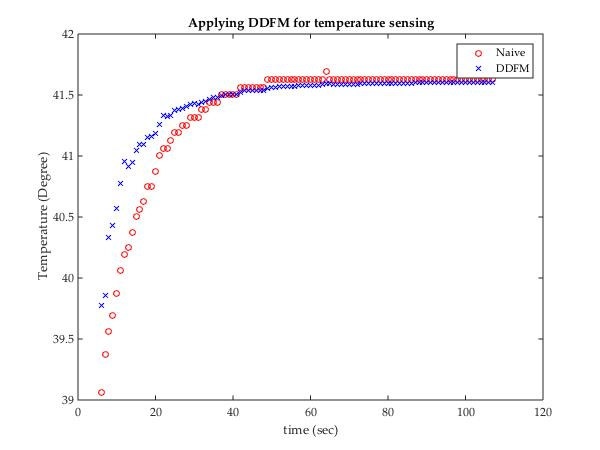
\includegraphics[width=0.5\textwidth]{fig1_appDDFM.jpg}
    \caption{Applying DDFM for temperature sensing}
    \label{fig:appDDFM}
\end{figure}

\begin{figure}[!t]
    \centering
        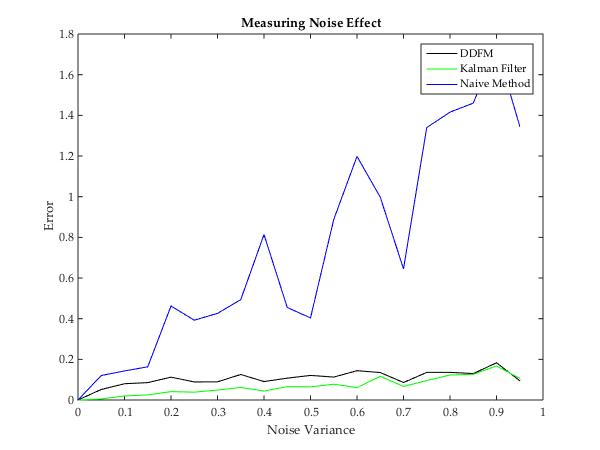
\includegraphics[width=0.5\textwidth]{fig2_noiseComp.jpg}
    \caption{Noise Effect Compare}
    \label{fig:noiseComp}
\end{figure}
\begin{figure}[!t]
    \centering
        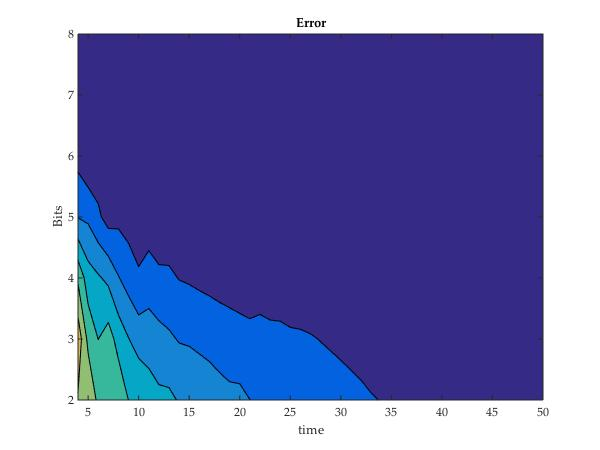
\includegraphics[width=0.5\textwidth]{fig3_bitsErr.jpg}
    \caption{Noise Effect Compare}
    \label{fig:noiseComp}
\end{figure}
\begin{figure}[!t]
    \centering
        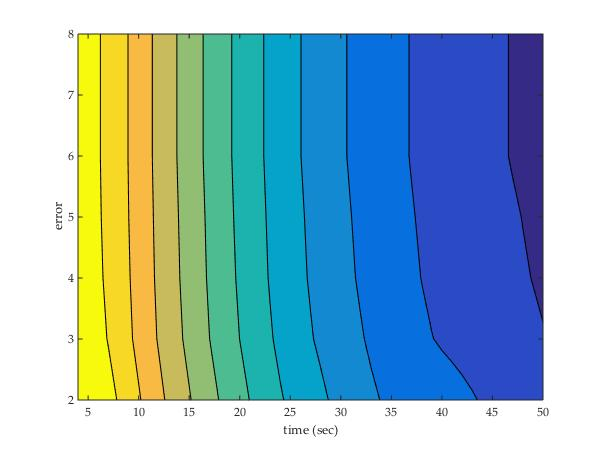
\includegraphics[width=0.5\textwidth]{fig4_bitsFiltered.jpg}
    \caption{Noise Effect Compare}
    \label{fig:noiseComp}
\end{figure}
\begin{figure}[!t]
    \centering
        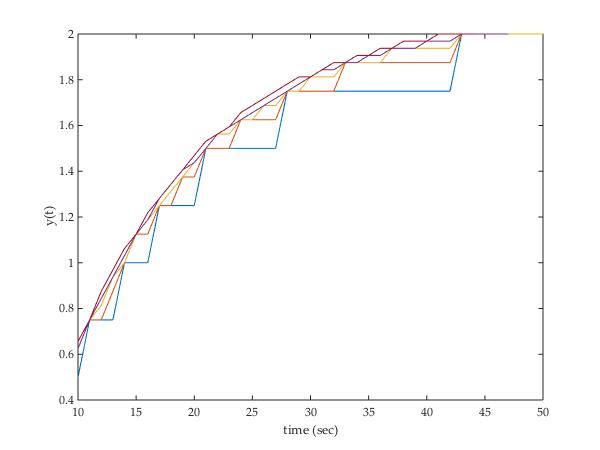
\includegraphics[width=0.5\textwidth]{fig5_quant.jpg}
    \caption{Noise Effect Compare}
    \label{fig:noiseComp}
\end{figure}
%\begin{figure}[!t]
%\centering
%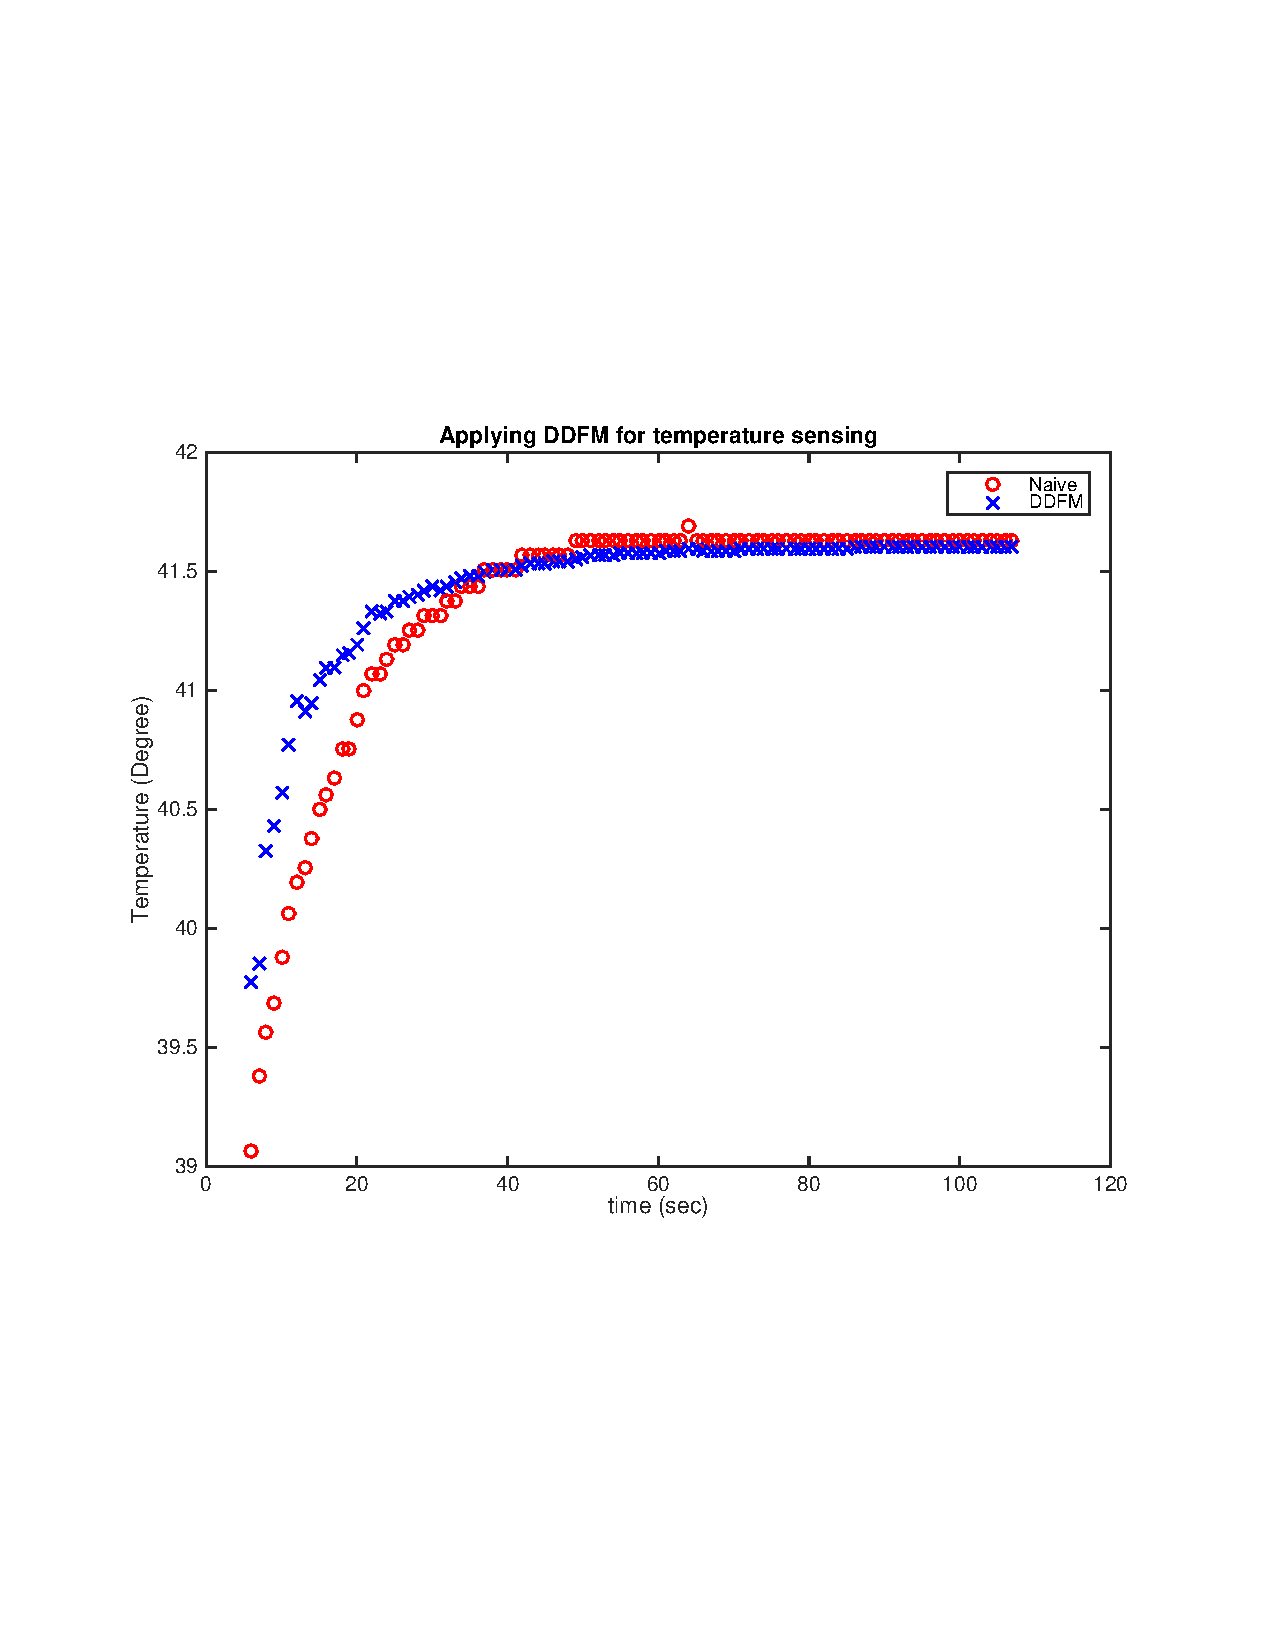
\includegraphics[width=4in]{fig1_appDDFM.pdf}
%\caption{Simulation results for the network.}
%\label{fig_sim}
%\end{figure}

% Note that the IEEE typically puts floats only at the top, even when this
% results in a large percentage of a column being occupied by floats.


%An example of a double column floating figure using two subfigures.
%(The subfig.sty package must be loaded for this to work.)
%The subfigure \label commands are set within each subfloat command,
%and the \label for the overall figure must come after \caption.
%\hfil is used as a separator to get equal spacing.
%Watch out that the combined width of all the subfigures on a 
%line do not exceed the text width or a line break will occur.

%\begin{figure*}[!t]
%\centering
%\subfloat[Case I]{\includegraphics[width=2.5in]{box}%
%\label{fig_first_case}}
%\hfil
%\subfloat[Case II]{\includegraphics[width=2.5in]{box}%
%\label{fig_second_case}}
%\caption{Simulation results for the network.}
%\label{fig_sim}
%\end{figure*}
%
% Note that often IEEE papers with subfigures do not employ subfigure
% captions (using the optional argument to \subfloat[]), but instead will
% reference/describe all of them (a), (b), etc., within the main caption.
% Be aware that for subfig.sty to generate the (a), (b), etc., subfigure
% labels, the optional argument to \subfloat must be present. If a
% subcaption is not desired, just leave its contents blank,
% e.g., \subfloat[].


% An example of a floating table. Note that, for IEEE style tables, the
% \caption command should come BEFORE the table and, given that table
% captions serve much like titles, are usually capitalized except for words
% such as a, an, and, as, at, but, by, for, in, nor, of, on, or, the, to
% and up, which are usually not capitalized unless they are the first or
% last word of the caption. Table text will default to \footnotesize as
% the IEEE normally uses this smaller font for tables.
% The \label must come after \caption as always.
%
%\begin{table}[!t]
%% increase table row spacing, adjust to taste
%\renewcommand{\arraystretch}{1.3}
% if using array.sty, it might be a good idea to tweak the value of
% \extrarowheight as needed to properly center the text within the cells
%\caption{An Example of a Table}
%\label{table_example}
%\centering
%% Some packages, such as MDW tools, offer better commands for making tables
%% than the plain LaTeX2e tabular which is used here.
%\begin{tabular}{|c||c|}
%\hline
%One & Two\\
%\hline
%Three & Four\\
%\hline
%\end{tabular}
%\end{table}


% Note that the IEEE does not put floats in the very first column
% - or typically anywhere on the first page for that matter. Also,
% in-text middle ("here") positioning is typically not used, but it
% is allowed and encouraged for Computer Society conferences (but
% not Computer Society journals). Most IEEE journals/conferences use
% top floats exclusively. 
% Note that, LaTeX2e, unlike IEEE journals/conferences, places
% footnotes above bottom floats. This can be corrected via the
% \fnbelowfloat command of the stfloats package.



\section{Conclusion}
The conclusion goes here.



% if have a single appendix:
%\appendix[Proof of the Zonklar Equations]
% or
%\appendix  % for no appendix heading
% do not use \section anymore after \appendix, only \section*
% is possibly needed

% use appendices with more than one appendix
% then use \section to start each appendix
% you must declare a \section before using any
% \subsection or using \label (\appendices by itself
% starts a section numbered zero.)
%
\section{Contribution Summery}
% use section* for acknowledgment

%
\appendices
\section{Environment Introduction}
\subsection{LEGO EV3}
Lego Mindstorms EV3 is the third generation robotics kit in Lego's Mindstorms line. It is the successor to the second generation Lego Mindstorms NXT 2.0 kit. The LEGO EV3 main processor is TI Sitara AM1808(ARM926EJ-S core) with clock frequency 300 MHz, for memory, it equips 64 MB RAM with 16 MB Flash.\cite{lego-intro}
\subsection{MATLAB Interface}
MATLAB\textregistered  Support Package for LEGO\textregistered MINDSTORMS EV3 Hardware is a support package developed and supported by MATLAB\textregistered group to control LEGO\textregistered MINDSTORMS EV3 robots. The support package provides MATLAB functions to control the motors and interface with the hardware input sensors and output capabilities. 
%
%% you can choose not to have a title for an appendix
%% if you want by leaving the argument blank
%\section{}
%Appendix two text goes here.


\section*{Acknowledgment}


The author would like to thank Prof. Ivan for his kind help in the research and the essay writing. He is always patient and inspiring.


% Can use something like this to put references on a page
% by themselves when using endfloat and the captionsoff option.
\ifCLASSOPTIONcaptionsoff
  \newpage
\fi



% trigger a \newpage just before the given reference
% number - used to balance the columns on the last page
% adjust value as needed - may need to be readjusted if
% the document is modified later
%\IEEEtriggeratref{8}
% The "triggered" command can be changed if desired:
%\IEEEtriggercmd{\enlargethispage{-5in}}

% references section

\bibliographystyle{IEEEtran}
\bibliography{./ref/reportlib} 

% can use a bibliography generated by BibTeX as a .bbl file
% BibTeX documentation can be easily obtained at:
% http://mirror.ctan.org/biblio/bibtex/contrib/doc/
% The IEEEtran BibTeX style support page is at:
% http://www.michaelshell.org/tex/ieeetran/bibtex/
%\bibliographystyle{IEEEtran}
% argument is your BibTeX string definitions and bibliography database(s)
%\bibliography{IEEEabrv,../bib/paper}
%
% <OR> manually copy in the resultant .bbl file
% set second argument of \begin to the number of references
% (used to reserve space for the reference number labels box)
%\begin{thebibliography}{1}
%
%\bibitem{IEEEhowto:kopka}
%H.~Kopka and P.~W. Daly, \emph{A Guide to \LaTeX}, 3rd~ed.\hskip 1em plus
%  0.5em minus 0.4em\relax Harlow, England: Addison-Wesley, 1999.
%
%\end{thebibliography}

% biography section
% 
% If you have an EPS/PDF photo (graphicx package needed) extra braces are
% needed around the contents of the optional argument to biography to prevent
% the LaTeX parser from getting confused when it sees the complicated
% \includegraphics command within an optional argument. (You could create
% your own custom macro containing the \includegraphics command to make things
% simpler here.)
%\begin{IEEEbiography}[{\includegraphics[width=1in,height=1.25in,clip,keepaspectratio]{mshell}}]{Michael Shell}
% or if you just want to reserve a space for a photo:

%\begin{IEEEbiography}{Michael Shell}
%Biography text here.
%\end{IEEEbiography}

% if you will not have a photo at all:
%\begin{IEEEbiographynophoto}{John Doe}
%Biography text here.
%\end{IEEEbiographynophoto}

% insert where needed to balance the two columns on the last page with
% biographies
%\newpage

%\begin{IEEEbiographynophoto}{Jane Doe}
%Biography text here.
%\end{IEEEbiographynophoto}

% You can push biographies down or up by placing
% a \vfill before or after them. The appropriate
% use of \vfill depends on what kind of text is
% on the last page and whether or not the columns
% are being equalized.

%\vfill

% Can be used to pull up biographies so that the bottom of the last one
% is flush with the other column.
%\enlargethispage{-5in}



% that's all folks
\end{document}


